\begin{figure}[H]
\centering
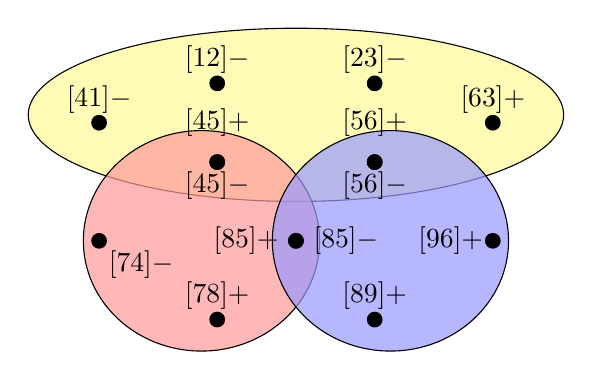
\begin{tikzpicture}
    \node (v12) at (1.5,3.5) {};
    \node (v23) at (3.5, 3.5) {};
    \node (v41) at (0, 3) {};
    \node (v63) at (5,3) {};
    \node (v45) at (1.5,2.5) {};
    \node (v56) at (3.5,2.5) {};
    \node (v74) at (0,1.5) {};
    \node (v85) at (2.5,1.5) {};
    \node (v96) at (5,1.5) {};
    \node (v78) at (1.5,0.5) {};
    \node (v89) at (3.5,0.5) {};

    \begin{scope}[fill opacity=0.7]
     \filldraw[fill=yellow!40] (2.5, 3.1) ellipse [x radius=3.4, y radius=1.1];
    \filldraw[fill=red!40] (1.3, 1.5) ellipse [rotate=0, x radius=1.5, y radius=1.4];
     \filldraw[fill=blue!40] (3.7, 1.5) ellipse [rotate=0, x radius=1.5, y radius=1.4];
    \end{scope}
    
    \fill (v12) circle (0.1) node [above] {$[12]-$};
    \fill (v23) circle (0.1) node [above] {$[23]-$};
    \fill (v41) circle (0.1) node [above] {$[41]-$};
    \fill (v63) circle (0.1) node [above] {$[63]+$};
    \fill (v45) circle (0.1) node [above=0.2cm] {$[45]+$};
    \fill (v45) circle (0.1) node [below] {$[45]-$};
    \fill (v56) circle (0.1) node [above=0.2cm] {$[56]+$}; %below left
    \fill (v56) circle (0.1) node [below] {$[56]-$};
    \fill (v74) circle (0.1) node [below right] {$[74]-$};
    %\fill (v74) circle (0.1) node [right] {$-$};
    \fill (v85) circle (0.1) node [left=0.1cm] {$[85]+$};
    \fill (v85) circle (0.1) node [right=0.1cm] {$[85]-$};
    %\fill (v85) circle (0.1) node [left=0.2cm] {$+$};
    \fill (v96) circle (0.1) node [left] {$[96]+$};
    \fill (v78) circle (0.1) node [above] {$[78]+$};
    \fill (v89) circle (0.1) node [above] {$[89]+$};
    % \node at (0.2,2.8) {$e_1$};
    % \node at (2.3,3) {$e_2$};
    % \node at (3,0.8) {$e_3$};
    % \node at (0.1,0.7) {$e_4$};
\end{tikzpicture}
\caption{\footnotesize{The oriented hypergraph $\widetilde{\KK}$,
which contains three hyperedges $e_1, e_2, e_3$,
with $e_1=\{[12]-, [23]-, [41]-, [63]+, [45]+, [56]+\}$,
$e_2=\{[45]-, [74]-, [85]+, [78]+\}$,
and
$e_3=\{[56]-, [85]-, [96]+, [89]+\}$.
}}
\label{fig_hyp_grph_1}
\end{figure}